% ============================================================================
% BUKU PANDUAN PENGGUNAAN SISTEM (MANUAL BOOK)
% Universitas Gunadarma
%
% Judul: BUKU PANDUAN PENGGUNAAN SISTEM DETEKSI AREA INFEKSI PNEUMONIA
%        PADA CITRA RONTGEN DADA MENGGUNAKAN ARSITEKTUR U-NET BERBASIS
%        CONVOLUTIONAL NEURAL NETWORK (CNN)
%
% Penulis  : Muhammad Hisyam (NPM: 51422075)
% Pembimbing: Dr. Tavipia Rumambi, SKom., MMSI.
%
% Format Penulisan Sesuai Ketentuan Universitas Gunadarma:
% - Font    : Calibri / Sans-Serif (12pt)
% - Margin  : Atas 4cm, Kiri 4cm, Bawah 3cm, Kanan 3cm
% - Spasi   : 1.5
% ============================================================================
\documentclass[12pt,a4paper]{article}

% --- Packages ---------------------------------------------------------------
\usepackage[T1]{fontenc}
\usepackage[utf8]{inputenc}
\usepackage[indonesian]{babel}
\usepackage{helvet}
\renewcommand{\familydefault}{\sfdefault}

\usepackage{geometry}
\geometry{
    a4paper,
    top        = 4cm,
    left       = 4cm,
    bottom     = 3cm,
    right      = 3cm,
    headheight = 14pt
}

\usepackage{setspace}
\onehalfspacing

\usepackage{graphicx}
\graphicspath{{../img/}{../../doc/img/}{img/}}

\usepackage{booktabs}
\usepackage{tabularx}
\usepackage{multirow}
\usepackage{array}
\usepackage{xcolor}
\usepackage{float}
\usepackage{listings}
\usepackage{titlesec}
\usepackage{fancyhdr}
\usepackage{hyperref}
\usepackage{enumitem}
\usepackage{caption}

% --- Section Formatting -----------------------------------------------------
\titleformat{\section}[block]
    {\normalfont\large\bfseries}
    {\roman{section}.}{0.8em}{}
\titlespacing*{\section}{0pt}{18pt}{8pt}

\titleformat{\subsection}[block]
    {\normalfont\bfseries}
    {\arabic{section}.\arabic{subsection}}{0.6em}{}
\titlespacing*{\subsection}{0pt}{12pt}{6pt}

\titleformat{\subsubsection}[block]
    {\normalfont\bfseries\itshape}
    {\arabic{section}.\arabic{subsection}.\arabic{subsubsection}}{0.6em}{}
\titlespacing*{\subsubsection}{0pt}{10pt}{4pt}

% --- Caption Formatting -----------------------------------------------------
\captionsetup{font=small, labelfont=bf, skip=6pt}

% --- Listings Setup ---------------------------------------------------------
\lstset{
    basicstyle       = \ttfamily\small,
    keywordstyle     = \color{black}\bfseries,
    commentstyle     = \color{gray},
    stringstyle      = \color{black},
    breaklines       = true,
    frame            = single,
    backgroundcolor  = \color{gray!8},
    numbers          = none,
    showstringspaces = false,
    tabsize          = 2,
    xleftmargin      = 4pt,
    xrightmargin     = 4pt
}

% --- Hyperlink Setup --------------------------------------------------------
\hypersetup{
    colorlinks  = true,
    linkcolor   = black,
    citecolor   = black,
    urlcolor    = black
}

% --- Header/Footer ----------------------------------------------------------
\pagestyle{fancy}
\fancyhf{}
\rhead{\small\itshape Buku Panduan Sistem Deteksi Pneumonia}
\lhead{\small\itshape Universitas Gunadarma}
\rfoot{\thepage}
\renewcommand{\headrulewidth}{0.4pt}
\renewcommand{\footrulewidth}{0.4pt}

\begin{document}

% ============================================================================
% i. COVER
% ============================================================================
\thispagestyle{empty}
\begin{center}
    \vspace*{1.2cm}

    {\fontsize{16pt}{20pt}\selectfont\bfseries
    DETEKSI AREA INFEKSI PNEUMONIA PADA CITRA RONTGEN DADA\\[6pt]
    MENGGUNAKAN ARSITEKTUR U-NET BERBASIS\\[6pt]
    CONVOLUTIONAL NEURAL NETWORK (CNN)\par}

    \vspace{2.2cm}

    % Logo Gunadarma
    
\includegraphics[width=5.5cm]{logo_gunadarma.png}

    \vspace{2.2cm}

    {\fontsize{12pt}{16pt}\selectfont
    Dibuat oleh :\\[8pt]
    \textbf{Muhammad Hisyam}\\[4pt]
    \textbf{Dr. Tavipia Rumambi, SKom., MMSI.}\par}

    \vspace{2.5cm}

    {\fontsize{14pt}{18pt}\selectfont\bfseries
    UNIVERSITAS GUNADARMA\\[4pt]
    2026\par}
\end{center}

\newpage
\setcounter{page}{1}
\setcounter{section}{1}

% ============================================================================
% ii. GAMBARAN UMUM APLIKASI
% ============================================================================
\section{Gambaran Umum Aplikasi}

\subsection{Latar Belakang dan Tujuan Aplikasi}

Pneumonia merupakan salah satu penyakit infeksi saluran pernapasan akut yang
memiliki tingkat kematian tinggi, khususnya pada anak-anak di bawah lima tahun,
lansia, dan pasien dengan imunitas rendah. Berdasarkan data \textit{World Health
Organization} (WHO), penyakit ini merenggut sekitar 2,5 juta jiwa di seluruh
dunia pada tahun 2019. Secara klinis, diagnosis awal umumnya mengandalkan
pemeriksaan citra radiografi dada (\textit{Chest X-Ray}/CXR). Namun, proses
pembacaan citra rontgen secara manual memerlukan keahlian spesialis radiologi,
menghabiskan waktu 15--60 menit per kasus, dan memiliki risiko kesalahan
interpretasi hingga 15--20\% di fasilitas dengan keterbatasan tenaga ahli.

Aplikasi Web Deteksi Pneumonia ini dibangun sebagai alat bantu keputusan medis
berbasis komputer (\textit{Computer-Aided Diagnosis}/CAD) yang memanfaatkan
teknologi kecerdasan buatan (\textit{Deep Learning}). Aplikasi ini dirancang
untuk melakukan segmentasi otomatis area infeksi pneumonia pada citra rontgen
dada, mengklasifikasikan derajat keparahan infeksi ke dalam 5 tingkatan klinis,
menentukan lokasi sebaran (lateralitas), serta memberikan visualisasi transparansi
keputusan model berbasis \textit{Explainable AI} (XAI/Grad-CAM).

\subsection{Arsitektur dan Teknologi Inti}

Aplikasi ini dikembangkan berbasis arsitektur modular yang terdiri dari empat
komponen utama yang terintegrasi penuh (Gambar~\ref{fig:arsitektur_sistem}).

\begin{figure}[H]
  \centering
  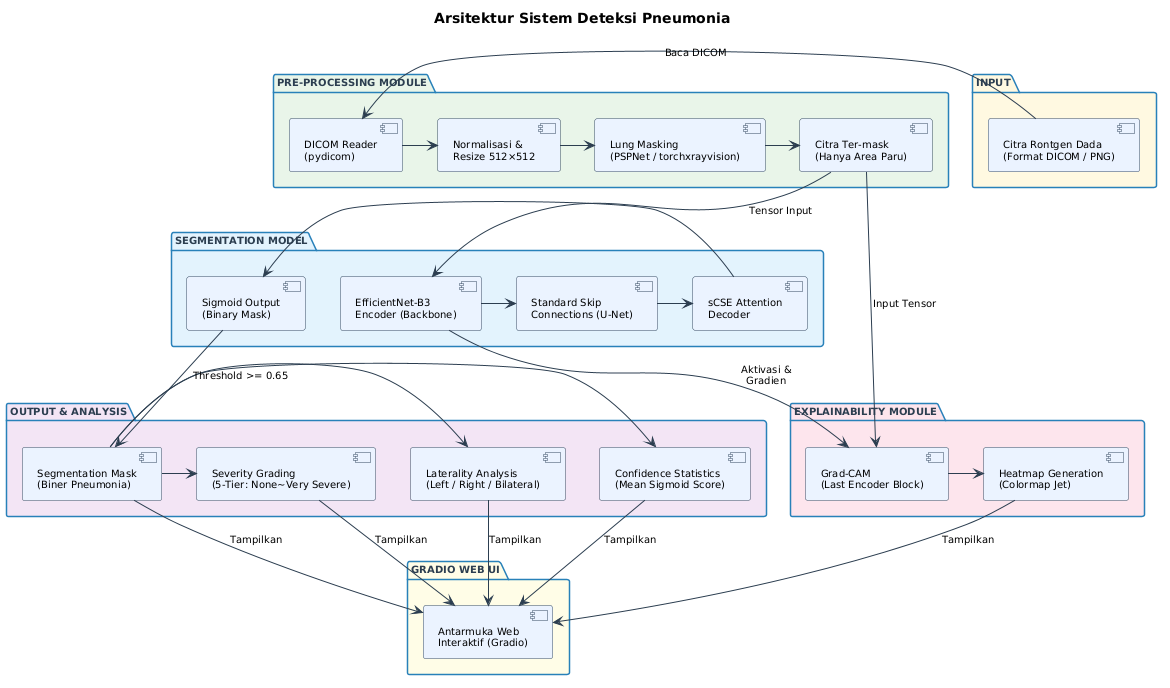
\includegraphics[width=0.92\textwidth,keepaspectratio]{arsitektur_sistem.png}
  \caption{Diagram Arsitektur Sistem Deteksi Pneumonia Empat Modul.}
  \label{fig:arsitektur_sistem}
\end{figure}

\begin{enumerate}
    \item \textbf{Modul Pra-pemrosesan \& Segmentasi Paru-Paru
    (\textit{Lung Masking})}: Membaca berkas medis DICOM atau citra digital,
    melakukan penyesuaian kontras (CLAHE), dan secara otomatis memotong area
    organ paru-paru menggunakan model PSPNet dari pustaka
    \texttt{torchxrayvision}. Proses ini mengeliminasi bayangan organ di luar
    paru-paru, tulang rusuk luar, serta teks radiologi agar model utama tidak
    mengalami kegagalan generalisasi.

    \item \textbf{Modul Segmentasi U-Net sCSE}: Menggunakan model jaringan
    saraf konvolusional arsitektur U-Net dengan mekanisme atensi \textit{Spatial
    and Channel Squeeze-and-Excitation} (sCSE) dan pengekstrak fitur
    (\textit{encoder}) \textit{EfficientNet-B3} yang dipra-latih pada ImageNet.
    Model dilatih menggunakan dataset \textit{RSNA Pneumonia Detection Challenge}
    (26.684 citra DICOM) dengan fungsi kerugian \textit{Unified Focal Loss} dan
    optimizer AdamW, menghasilkan performa terbaik: Dice \textbf{0,6234},
    Precision \textbf{0,6868}, Recall \textbf{0,7082}, dan Specificity
    \textbf{0,9781}.

    \item \textbf{Modul Keterjelasan Model (\textit{Grad-CAM})}: Menghasilkan
    peta panas (\textit{heatmap}) gradien lokal berbasis \textit{Gradient-weighted
    Class Activation Mapping} untuk menunjukkan area mana yang menjadi fokus
    utama jaringan saraf dalam mendeteksi infeksi, meningkatkan kepercayaan klinis
    terhadap keputusan model.

    \item \textbf{Modul Antarmuka Web Gradio \& Cloudflare Tunnel}: Menyediakan
    antarmuka grafik interaktif yang dapat digunakan tenaga medis melalui
    peramban web, serta mendukung akses publik melalui koneksi terenkripsi
    Cloudflare Tunnel (\url{https://grad.mhisyam.com}).
\end{enumerate}

\subsection{Skema Penyebaran Publik (Cloudflare Tunnel)}

Untuk memungkinkan tenaga medis mengakses aplikasi dari luar jaringan lokal
tanpa membuka port firewall, digunakan arsitektur hybrid berbasis Cloudflare
Tunnel (Gambar~\ref{fig:cloudflare_tunnel}). Daemon \texttt{cloudflared} yang
berjalan pada server lokal membangun terowongan terenkripsi keluar menuju
jaringan Anycast Cloudflare, sehingga semua permintaan HTTPS dari klien
diteruskan secara aman ke \texttt{http://localhost:7860} tanpa memerlukan
konfigurasi \textit{port forwarding} atau IP publik statis.

\begin{figure}[H]
  \centering
  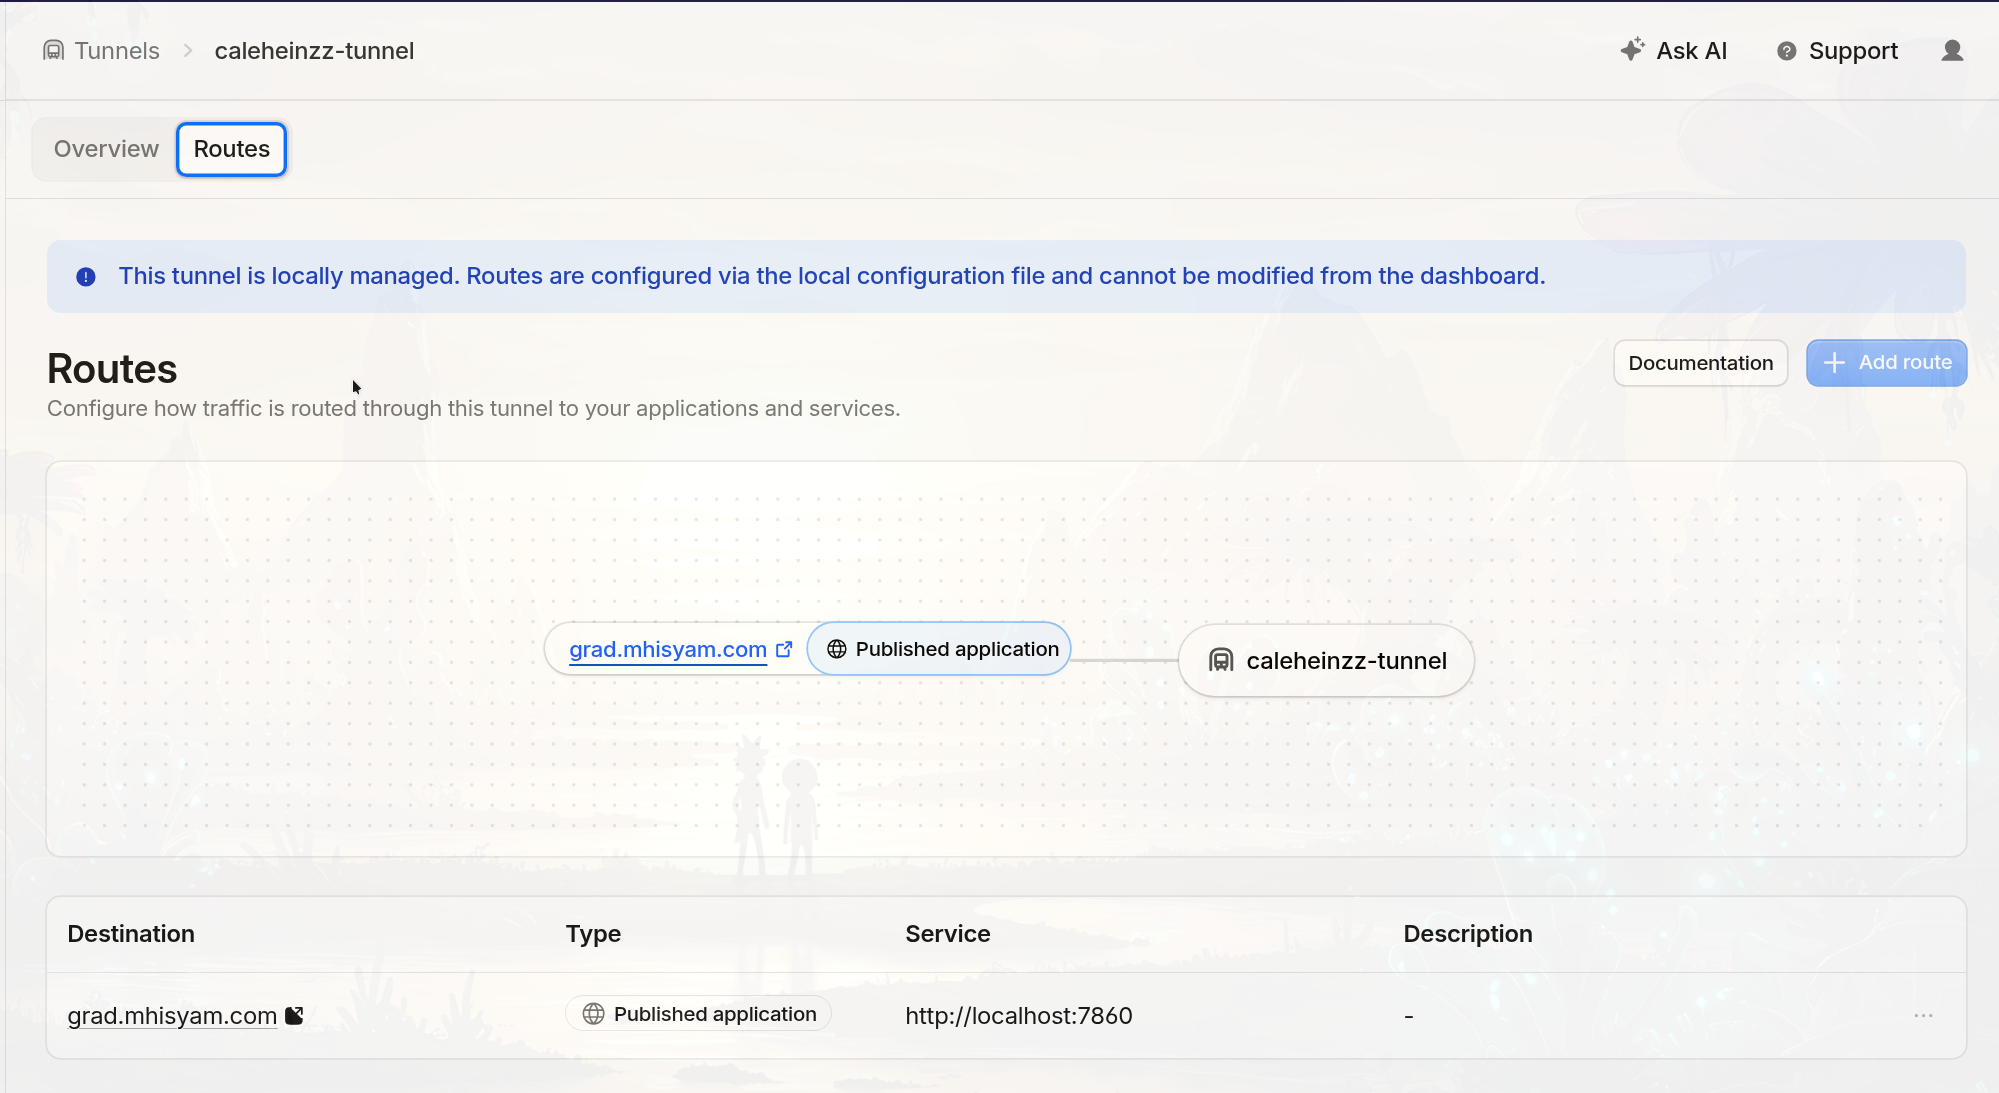
\includegraphics[width=0.88\textwidth,keepaspectratio]{cloudflare_tunnel.png}
  \caption{Skema Arsitektur Penyebaran Publik via Cloudflare Tunnel.}
  \label{fig:cloudflare_tunnel}
\end{figure}

\subsection{Fitur-Fitur Utama Aplikasi}

\begin{enumerate}
    \item \textbf{Dukungan Multi-Format Citra}: Menerima masukan berkas medis
    standar DICOM (\texttt{.dcm}) maupun berkas citra digital umum (\texttt{.png},
    \texttt{.jpg}, \texttt{.jpeg}, \texttt{.bmp}, \texttt{.tif}, \texttt{.webp}).

    \item \textbf{Dua Mode Pengunggahan}: Tab \textit{File Upload} untuk DICOM
    dan citra, serta tab \textit{Drag \& Drop Gambar} untuk mengunggah langsung
    dengan cara menyeret gambar ke area antarmuka.

    \item \textbf{Kontrol Sensitivitas Threshold}: Slider ambang batas
    probabilitas ($0{,}10$ hingga $0{,}90$, bawaan $0{,}65$) yang dapat
    disesuaikan pengguna secara \textit{real-time} untuk mengatur keseimbangan
    Presisi vs.\ Sensitivitas.

    \item \textbf{Keluaran Visual Grid 2$\times$2}: Menyajikan empat tampilan
    visual terintegrasi sekaligus: (A)~Overlay Infeksi merah, (B)~Heatmap
    Grad-CAM berwarna JET, (C)~Masker Paru biner PSPNet, dan (D)~Paru Terisolasi.

    \item \textbf{Klasifikasi Keparahan 5 Tingkatan}: Normal, Ringan ($\le5\%$),
    Sedang ($5\%$--$15\%$), Berat ($15\%$--$30\%$), dan Kritis ($>30\%$)
    berdasarkan rasio piksel infeksi terhadap total parenkim paru.

    \item \textbf{Analisis Lateralitas Infeksi}: Mengidentifikasi sebaran lesi
    pada Paru Kanan (\textit{Right-Sided}), Paru Kiri (\textit{Left-Sided}),
    atau Kedua Paru (\textit{Bilateral}), beserta distribusi zona atas dan bawah.

    \item \textbf{Dashboard KPI Real-Time}: Kartu ringkasan status deteksi
    (NORMAL/PNEUMONIA), rasio infeksi (\%), tingkat keparahan, dan
    \textit{confidence score} (rata-rata, maksimum, minimum, standar deviasi).

    \item \textbf{Citra Contoh Preset}: Contoh citra rontgen bawaan (Normal,
    Pneumonia Bakteri, Pneumonia Virus) untuk pengujian cepat tanpa perlu
    mengunggah berkas.

    \item \textbf{Kecepatan Inferensi Tinggi}: Seluruh \textit{pipeline}
    inferensi (PSPNet masking + U-Net sCSE + Grad-CAM) selesai dalam
    \textbf{1--3 detik} per citra pada GPU NVIDIA RTX 3070 Laptop (8 GB VRAM).

    \item \textbf{Inferensi Prediksi via CLI}: Selain antarmuka web, sistem
    mendukung prediksi tunggal maupun prediksi \textit{batch} melalui
    \textit{command-line interface} (CLI).
\end{enumerate}


% ============================================================================
% iii. KEBUTUHAN HARDWARE DAN SOFTWARE
% ============================================================================
\section{Kebutuhan Hardware dan Software}

Untuk menjalankan dan mengakses aplikasi ini dengan optimal, berikut adalah
spesifikasi perangkat keras (\textit{hardware}) dan perangkat lunak
(\textit{software}) yang dibutuhkan.

\subsection{Kebutuhan Server (Lingkungan Eksekusi Model)}

Server bertindak sebagai mesin yang menampung model \textit{deep learning} dan
melayani proses inferensi secara lokal maupun publik.

\begin{table}[H]
\centering
\caption{Spesifikasi Kebutuhan Hardware Server}
\begin{tabularx}{\textwidth}{l X X}
\toprule
\textbf{Komponen} & \textbf{Kebutuhan Minimum} & \textbf{Rekomendasi Terbaik} \\
\midrule
Prosesor (CPU)     & Intel Core i5 / AMD Ryzen 5 (4 Core)       & AMD Ryzen 7 5800H / Intel i7-12700H (8+ Core) \\
Memori (RAM)       & 16 GB DDR4                                  & 32 GB DDR4 \\
Kartu Grafis (GPU) & NVIDIA GTX 1660 Ti (6 GB VRAM)              & NVIDIA RTX 3070 / RTX 3060 (8 GB VRAM) \\
Penyimpanan        & SSD 15 GB ruang kosong                      & NVMe SSD 30 GB ruang kosong \\
Sistem Operasi     & Ubuntu 22.04 LTS / Windows 10 (WSL2)        & CachyOS / Ubuntu 24.04 LTS \\
\bottomrule
\end{tabularx}
\end{table}

\begin{table}[H]
\centering
\caption{Spesifikasi Kebutuhan Software Server}
\begin{tabularx}{\textwidth}{l X}
\toprule
\textbf{Perangkat Lunak}     & \textbf{Versi / Keterangan} \\
\midrule
Bahasa Pemrograman           & Python $\ge 3.10$ (disarankan Python 3.11) \\
Manajer Paket                & \texttt{uv} (sangat direkomendasikan) atau \texttt{pip} \\
Framework Deep Learning      & PyTorch $\ge 2.4.0$ + CUDA 12.x \\
Pustaka Segmentasi Medis     & \texttt{segmentation-models-pytorch} (SMP) \\
Pustaka Masking Paru         & \texttt{torchxrayvision} (PSPNet) \\
Pustaka Augmentasi           & \texttt{albumentations} $\ge 1.4.0$ \\
Pustaka Citra Medis          & \texttt{pydicom}, \texttt{opencv-python}, \texttt{Pillow} \\
Antarmuka Web                & \texttt{gradio} $\ge 5.0.0$ \\
Akses Publik (opsional)      & \texttt{cloudflared} (Cloudflare Tunnel CLI) \\
\bottomrule
\end{tabularx}
\end{table}

\subsection{Kebutuhan Alternatif: Docker (Opsional)}

Sebagai alternatif instalasi manual, aplikasi dapat dijalankan dalam wadah
Docker yang telah terkonfigurasi lengkap, membutuhkan komponen tambahan berikut:

\begin{table}[H]
\centering
\caption{Kebutuhan Tambahan untuk Deployment via Docker}
\begin{tabularx}{\textwidth}{l X}
\toprule
\textbf{Komponen} & \textbf{Keterangan} \\
\midrule
Docker Engine          & Docker Engine $\ge 20.10$ (Linux) atau Docker Desktop $\ge 4.x$ \\
NVIDIA Container Toolkit & \texttt{nvidia-container-toolkit} (diperlukan untuk akses GPU di dalam kontainer) \\
Ruang Disk Tambahan    & $\pm$8 GB untuk \textit{image} Docker \\
\bottomrule
\end{tabularx}
\end{table}

\subsection{Kebutuhan Perangkat Pengguna (Client)}

Pengguna akhir (dokter, radiolog, atau perawat) dapat mengakses aplikasi web
melalui perangkat apa pun tanpa perlu menginstal aplikasi tambahan.

\begin{table}[H]
\centering
\caption{Spesifikasi Kebutuhan Perangkat Pengguna (Client)}
\begin{tabularx}{\textwidth}{l X}
\toprule
\textbf{Komponen}        & \textbf{Spesifikasi} \\
\midrule
Perangkat                & Komputer PC, Laptop, Tablet, atau Smartphone \\
Peramban Web (Browser)   & Google Chrome, Mozilla Firefox, Microsoft Edge, atau Safari (versi terbaru) \\
Koneksi Internet         & Koneksi stabil (minimum 2 Mbps untuk akses publik) \\
Resolusi Layar           & Minimum $1024\times768$ piksel (Desktop) atau $360\times640$ (Mobile) \\
\bottomrule
\end{tabularx}
\end{table}


% ============================================================================
% iv. PETUNJUK INSTALASI
% ============================================================================
\section{Petunjuk Instalasi}

Bagian ini menjelaskan dua metode instalasi: \textbf{Metode A} (instalasi
manual menggunakan \texttt{uv}/\texttt{pip}) dan \textbf{Metode B} (menggunakan
Docker). Pengguna cukup memilih salah satu metode sesuai lingkungan servernya.

\subsection{Metode A: Instalasi Manual (Direkomendasikan)}

\subsubsection{Langkah 1: Mengunduh Repositori Kode Sumber}

Buka terminal pada server, lalu kloning repositori proyek:
\begin{lstlisting}[language=bash]
git clone https://github.com/louiscalvin/pneumonia-segmentation-unet.git
cd pneumonia-segmentation-unet
\end{lstlisting}

\subsubsection{Langkah 2: Menyiapkan Lingkungan Virtual Python}

Sangat disarankan menggunakan manajer paket \texttt{uv} untuk kecepatan
instalasi dan isolasi dependensi:
\begin{lstlisting}[language=bash]
# Menggunakan uv (direkomendasikan):
uv sync                         # Buat .venv dan instal semua dependensi otomatis
source .venv/bin/activate        # Linux / macOS
# .venv\Scripts\activate         # Windows

# Atau menggunakan python venv:
python3 -m venv .venv
source .venv/bin/activate
pip install -r requirements.txt
\end{lstlisting}

\subsubsection{Langkah 3: Menyiapkan Berkas Model Checkpoint}

Pastikan berkas bobot model terbaik (\texttt{best\_model.pth}) telah diletakkan
pada direktori yang sesuai konfigurasi \texttt{config.yaml}:
\begin{lstlisting}[language=bash]
# Struktur direktori checkpoint (wajib ada sebelum menjalankan aplikasi):
outputs/checkpoints/best_model.pth
\end{lstlisting}

\subsubsection{Langkah 4: Menjalankan Aplikasi Web Gradio}

Jalankan aplikasi web menggunakan salah satu perintah berikut:
\begin{lstlisting}[language=bash]
# Menggunakan uv run (direkomendasikan):
uv run python -m app.gradio_app

# Atau langsung:
python app.py
\end{lstlisting}

Setelah berhasil, terminal akan menampilkan:
\begin{lstlisting}
* Running on local URL:  http://0.0.0.0:7860
* Model UNet sCSE loaded from outputs/checkpoints/best_model.pth
\end{lstlisting}

Buka peramban web dan akses \url{http://localhost:7860}.

\subsubsection{Langkah 5: Menjalankan Cloudflare Tunnel (Opsional)}

Jika ingin aplikasi dapat diakses dari internet publik:
\begin{lstlisting}[language=bash]
cloudflared tunnel run --config cloudflared_config.json pneumonia-tunnel
\end{lstlisting}
Aplikasi kini dapat diakses secara terenkripsi HTTPS melalui:\\
\url{https://grad.mhisyam.com}

\subsection{Metode B: Instalasi via Docker}

Docker menyederhanakan instalasi dengan mengemas semua dependensi ke dalam satu
\textit{image} siap pakai. Pastikan Docker Engine dan NVIDIA Container Toolkit
telah terinstal di server.

\subsubsection{Langkah 1: Membangun Image Docker}

\begin{lstlisting}[language=bash]
# Dari direktori root proyek:
docker build -t pneumonia-unet:latest .
\end{lstlisting}

\subsubsection{Langkah 2: Menjalankan Kontainer Docker}

\begin{lstlisting}[language=bash]
# Jalankan kontainer dengan akses GPU dan port forwarding:
docker run --gpus all \
           -p 7860:7860 \
           -v $(pwd)/outputs:/app/outputs \
           pneumonia-unet:latest
\end{lstlisting}

\noindent Keterangan:
\begin{itemize}
    \item \texttt{--gpus all}: Mengaktifkan akses ke semua GPU NVIDIA yang tersedia.
    \item \texttt{-p 7860:7860}: Meneruskan port Gradio ke mesin host.
    \item \texttt{-v \$(pwd)/outputs:/app/outputs}: Memasang direktori checkpoint
    dari host ke dalam kontainer.
\end{itemize}

\subsection{Penjelasan Konfigurasi (\texttt{config.yaml})}

Berkas \texttt{config.yaml} di direktori root proyek mengatur seluruh perilaku
sistem, mulai dari pelatihan model hingga inferensi. Tabel berikut menjelaskan
parameter-parameter penting yang dapat disesuaikan:

\begin{table}[H]
\centering
\caption{Parameter Penting dalam \texttt{config.yaml}}
\begin{tabularx}{\textwidth}{l l X}
\toprule
\textbf{Seksi}   & \textbf{Parameter}           & \textbf{Nilai \& Keterangan} \\
\midrule
\texttt{model}   & \texttt{encoder\_name}       & \texttt{"timm-efficientnet-b3"} — \textit{backbone} encoder \\
                 & \texttt{decoder\_attention}  & \texttt{"scse"} — mekanisme atensi \\
\texttt{training}& \texttt{batch\_size}         & \texttt{8} — ukuran \textit{batch} fisik \\
                 & \texttt{encoder\_freeze}     & \texttt{12} — epoch \textit{warmup} encoder dibekukan \\
                 & \texttt{use\_amp}            & \texttt{true} — Automatic Mixed Precision (FP16) \\
\texttt{optimizer}& \texttt{lr}                 & \texttt{4.0e-4} — laju pembelajaran \textit{decoder} \\
                 & \texttt{encoder\_lr\_factor} & \texttt{0.02} — faktor pengali LR \textit{encoder} \\
\texttt{loss}    & \texttt{type}                & \texttt{"unified\_focal"} — fungsi kerugian \\
\texttt{inference}& \texttt{threshold}          & \texttt{0.65} — ambang batas probabilitas deteksi \\
                 & \texttt{use\_tta}            & \texttt{true} — \textit{Test-Time Augmentation} aktif \\
\texttt{app}     & \texttt{port}                & \texttt{7860} — port server Gradio \\
\bottomrule
\end{tabularx}
\end{table}

\subsection{Inferensi Prediksi via CLI (Opsional)}

Selain antarmuka web, sistem menyediakan antarmuka CLI untuk prediksi langsung
dari terminal, berguna untuk pemrosesan \textit{batch} otomatis:

\begin{lstlisting}[language=bash]
# Prediksi satu citra tunggal:
uv run python -m src.predict \
    --config config.yaml \
    --input data/sample.dcm

# Prediksi seluruh folder (batch):
uv run python -m src.predict \
    --config config.yaml \
    --input data/test_images/ \
    --output outputs/predictions/
\end{lstlisting}


% ============================================================================
% v. PETUNJUK PENGGUNA
% ============================================================================
\section{Petunjuk Pengguna}

Bagian ini memandu tenaga medis dalam menggunakan antarmuka aplikasi web Gradio
langkah demi langkah untuk melakukan analisis citra rontgen dada.

\subsection{Rancangan dan Tampilan Antarmuka Aplikasi}

Antarmuka aplikasi dirancang dengan tata letak dua kolom yang intuitif: kolom
kiri untuk panel masukan dan kontrol, serta kolom kanan untuk panel keluaran
visualisasi dan laporan diagnosis. Gambar~\ref{fig:rancangan_ui} menampilkan
rancangan antarmuka, dan Gambar~\ref{fig:implementasi_web_gradio} menampilkan
implementasi nyatanya.

\begin{figure}[H]
  \centering
  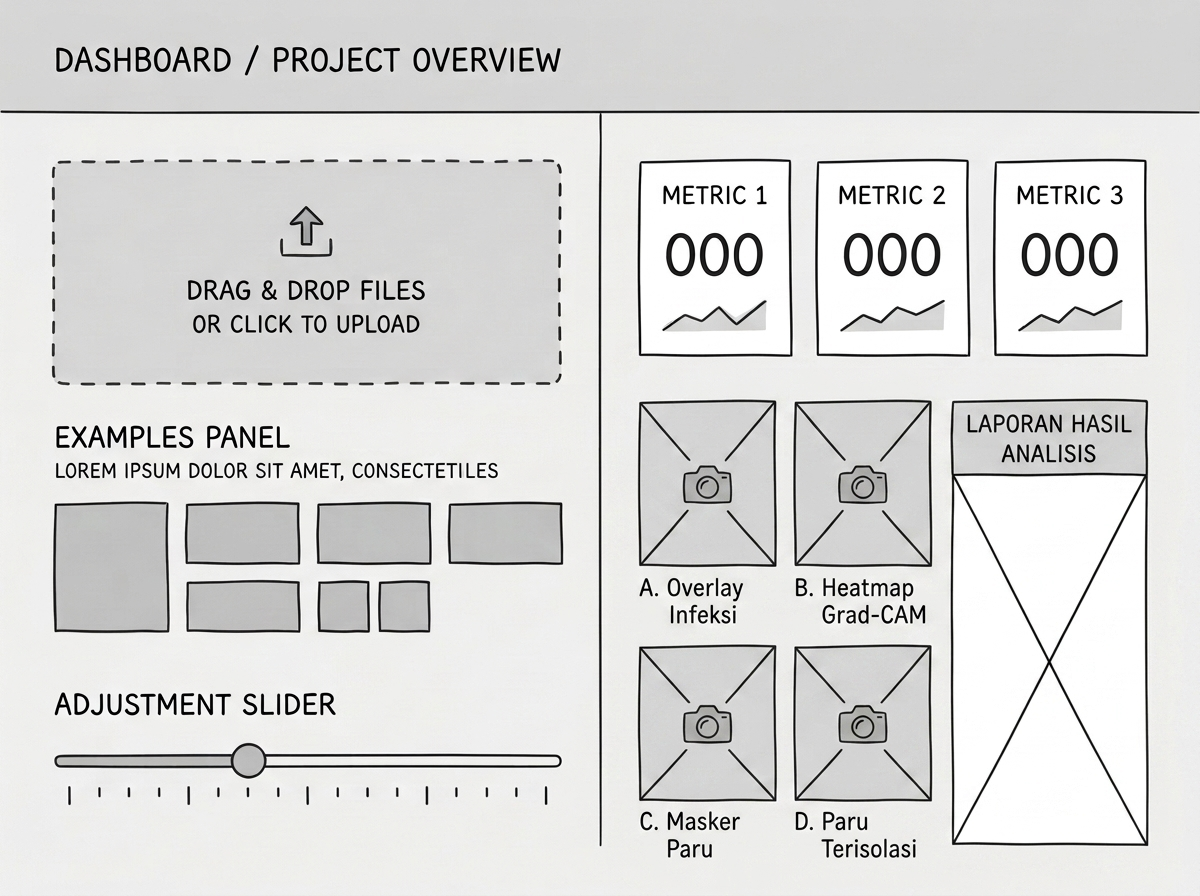
\includegraphics[width=0.9\textwidth,keepaspectratio]{rancangan_ui_web.jpg}
  \caption{Rancangan Antarmuka Web Aplikasi Deteksi Pneumonia.}
  \label{fig:rancangan_ui}
\end{figure}

\begin{figure}[H]
  \centering
  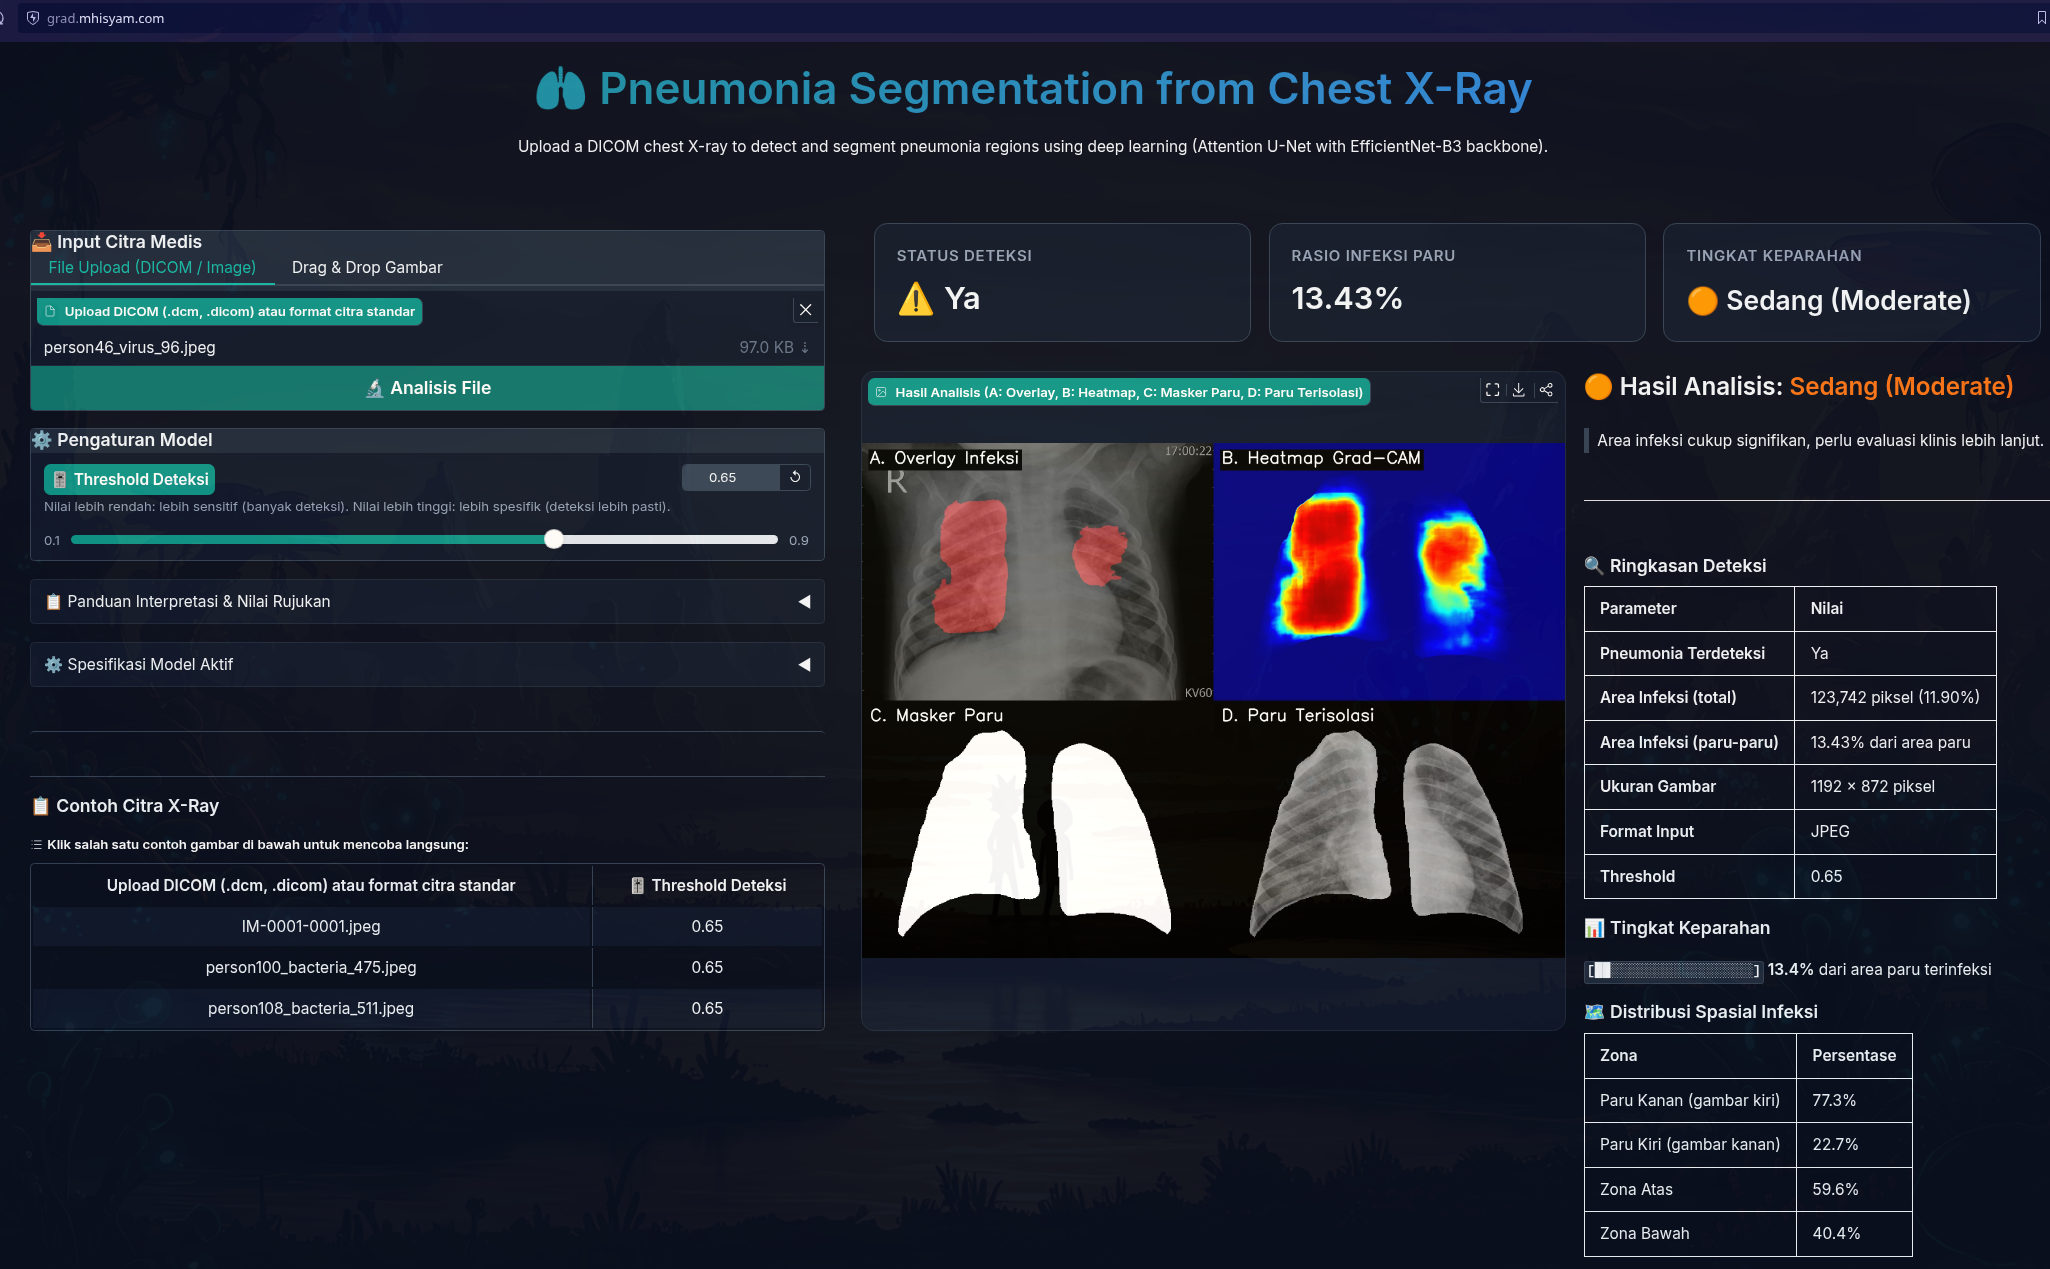
\includegraphics[width=\textwidth,keepaspectratio]{implementasi_web_gradio.png}
  \caption{Tampilan Implementasi Nyata Antarmuka Aplikasi Web Gradio.}
  \label{fig:implementasi_web_gradio}
\end{figure}

\subsection{Komponen Panel Kiri (Masukan \& Kontrol)}

\begin{enumerate}
    \item \textbf{Tab File Upload (DICOM / Image)}: Mode pengunggahan berkas
    medis DICOM (\texttt{.dcm}) maupun berkas citra standar (\texttt{.png},
    \texttt{.jpg}, dll.) menggunakan dialog pemilihan berkas. Tombol
    \textbf{``Analisis File''} digunakan untuk memulai analisis
    setelah berkas dipilih.

    \item \textbf{Tab Drag \& Drop Gambar}: Mode pengunggahan alternatif dengan
    cara menyeret dan menjatuhkan (\textit{drag and drop}) berkas gambar langsung
    ke area kotak yang tersedia. Tombol \textbf{``Analisis Gambar''}
    memulai analisis setelah gambar diletakkan.

    \item \textbf{Slider Threshold Deteksi} ($0{,}10$--$0{,}90$): Mengatur
    nilai ambang batas probabilitas piksel yang diklasifikasikan sebagai infeksi.
    Nilai \textit{default} adalah $\mathbf{0{,}65}$.

    \item \textbf{Accordion Panduan Interpretasi}: Panel yang dapat dibuka/ditutup
    berisi rujukan nilai keparahan (Normal, Ringan, Sedang, Berat, Kritis) serta
    panduan interpretasi visualisasi warna \textit{Overlay} Amber/Oranye dan
    \textit{Heatmap} termal medis INFERNO.

    \item \textbf{Accordion Spesifikasi Model Aktif}: Berisi informasi teknis
    model yang sedang aktif: arsitektur U-Net, \textit{encoder} EfficientNet-B3,
    mekanisme atensi sCSE, dan perangkat komputasi (CPU/GPU) yang digunakan.

    \item \textbf{Contoh Citra X-Ray (Preset)}: Kumpulan citra rontgen contoh
    yang dapat diklik langsung untuk pengujian cepat tanpa perlu mengunggah
    berkas dari komputer.
\end{enumerate}

\subsection{Komponen Panel Kanan (Dashboard \& Keluaran)}

\begin{enumerate}
    \item \textbf{Dashboard KPI}: Tiga kartu ringkasan yang tampil setelah
    analisis: (1)~Status Deteksi (NORMAL / PNEUMONIA), (2)~Rasio Infeksi Paru
    (\%), dan (3)~Tingkat Keparahan.

    \item \textbf{Grid Visual 2$\times$2}: Empat tampilan visual dalam satu
    gambar gabungan yang menampilkan hasil analisis dari berbagai sudut pandang (Overlay Amber, Heatmap INFERNO, Masker Paru, dan Paru Terisolasi).

    \item \textbf{Laporan Hasil Analisis}: Teks terstruktur berisi tabel
    ringkasan, distribusi spasial lesi, nilai kepercayaan statistik, serta
    keterangan medis.
\end{enumerate}

\subsection{Langkah-Langkah Penggunaan Aplikasi}

\subsubsection{1. Membuka Alamat Aplikasi}

Buka peramban web (Google Chrome/Firefox) dan masukkan salah satu alamat berikut:
\begin{itemize}
    \item \textbf{Akses Lokal (server lokal)}: \url{http://localhost:7860}
    \item \textbf{Akses Publik (internet)}: \url{https://grad.mhisyam.com}
\end{itemize}

\subsubsection{2. Memilih Mode dan Mengunggah Citra}

    \textbf{``Analisis File''}.
    \item \textbf{Tab ``Drag \& Drop Gambar''}: Seret dan jatuhkan berkas gambar
    ke area yang tersedia, lalu klik tombol \textbf{``Analisis Gambar''}.
    \item \textbf{Atau}: Klik salah satu gambar pada panel \textbf{Contoh Citra
    X-Ray} untuk langsung memuat citra uji bawaan.
\end{itemize}

\subsubsection{3. Mengatur Nilai Ambang Batas (\textit{Threshold})}

Sesuaikan \textit{slider} \textbf{Threshold Deteksi} sesuai kebutuhan klinis:
\begin{itemize}
    \item Nilai \textit{default} $\mathbf{0{,}65}$ optimal untuk keseimbangan
    Presisi dan Recall pada dataset RSNA.
    \item Geser ke \textbf{kiri} ($<0{,}50$) untuk meningkatkan sensitivitas
    (deteksi bercak infeksi yang sangat tipis/samar).
    \item Geser ke \textbf{kanan} ($>0{,}80$) untuk memperketat kepresisian dan
    menekan alarm palsu pada citra normal.
\end{itemize}

\subsubsection{4. Menjalankan Proses Analisis}

Klik tombol \textbf{``Analisis File''} atau \textbf{``Analisis Gambar''}
di bagian bawah panel masukan. Sistem akan memproses gambar melalui
\textit{pipeline} inferensi empat tahap selama \textbf{1--3 detik}.

\subsubsection{5. Mengamati Dashboard KPI}

Setelah selesai, tiga kartu KPI di atas panel kanan akan diperbarui:
\begin{itemize}
    \item \textbf{Status Deteksi}: Tidak Terdeteksi (NORMAL) atau Terdeteksi (PNEUMONIA).
    \item \textbf{Rasio Infeksi}: Persentase area infeksi terhadap total paru.
    \item \textbf{Tingkat Keparahan}: Label kelas keparahan dengan warna indikator.
\end{itemize}

\subsubsection{6. Mengamati Grid Visual 2$\times$2}

Panel kanan menampilkan satu gambar gabungan yang terdiri dari empat kuadran:
\begin{enumerate}
    \item \textbf{A. Overlay Infeksi (kiri atas)}: Citra rontgen asli dengan
    arsiran merah transparan ($\alpha=0{,}4$) pada area piksel infeksi yang
    diprediksi model.
    \item \textbf{B. Heatmap Grad-CAM (kanan atas)}: Peta panas gradasi warna
    JET (merah = fokus perhatian model tertinggi, biru = area netral).
    \item \textbf{C. Masker Paru PSPNet (kiri bawah)}: Citra biner hitam-putih
    hasil isolasi organ paru-paru oleh model PSPNet.
    \item \textbf{D. Paru Terisolasi (kanan bawah)}: Citra rontgen setelah area
    di luar paru-paru dihapus oleh masker PSPNet.
\end{enumerate}

\subsubsection{7. Membaca Laporan Ringkasan Kuantitatif}

Di bawah grid visual, sistem menyajikan laporan diagnosis terstruktur:
\begin{itemize}
    \item \textbf{Status \& Keparahan}: Tabel ringkasan status, derajat keparahan,
    rasio infeksi, dimensi citra, dan nilai threshold yang digunakan.
    \item \textbf{Distribusi Spasial}: Persentase infeksi pada paru kanan vs.\
    kiri, zona atas vs.\ bawah, serta diagnosis lateralitas (\textit{Right-Sided},
    \textit{Left-Sided}, atau \textit{Bilateral}).
    \item \textbf{Statistik Kepercayaan}: Nilai rata-rata, maksimum, minimum, dan
    standar deviasi probabilitas piksel infeksi.
\end{itemize}

Tabel~\ref{tab:severity} menjelaskan referensi nilai derajat keparahan yang
digunakan sistem:

\begin{table}[H]
\centering
\caption{Tabel Klasifikasi Derajat Keparahan Infeksi Pneumonia}
\label{tab:severity}
\begin{tabularx}{\textwidth}{l l X}
\toprule
\textbf{Tingkat}      & \textbf{Rasio Infeksi}  & \textbf{Interpretasi Klinis} \\
\midrule
Normal                & $0\%$                   & Tidak ada lesi infeksi terdeteksi. \\
Ringan (\textit{Mild})     & $>0\%$ s.d.\ $\le5\%$   & Infeksi lokal tahap awal; perlu observasi. \\
Sedang (\textit{Moderate}) & $>5\%$ s.d.\ $\le15\%$  & Lesi signifikan; evaluasi klinis segera. \\
Berat (\textit{Severe})    & $>15\%$ s.d.\ $\le30\%$ & Lesi ekstensif; konsultasi dokter mendesak. \\
Kritis (\textit{Critical}) & $>30\%$                 & Infeksi masif; penanganan darurat diperlukan. \\
\bottomrule
\end{tabularx}
\end{table}

\subsubsection{8. Mereset Antarmuka}

Untuk mengosongkan semua panel masukan dan keluaran sebelum menganalisis citra
pasien baru, klik ikon \textbf{$\times$} (hapus) pada komponen gambar masukan
atau muat ulang halaman di peramban.

\subsection{Hasil Pengujian Fungsionalitas (Black-Box Testing)}

Tabel berikut menrangkum hasil pengujian fungsionalitas sistem yang telah
dilakukan untuk memvalidasi seluruh fitur utama aplikasi:

\begin{table}[H]
\centering
\caption{Hasil Pengujian Fungsionalitas (Black-Box Testing) Aplikasi Web}
\begin{tabularx}{\textwidth}{c p{3cm} X X c}
\toprule
\textbf{No} & \textbf{Fitur / Fungsi} & \textbf{Skenario Input} & \textbf{Hasil yang Diharapkan} & \textbf{Status} \\
\midrule
1 & Pengunggahan Citra Valid      & Unggah berkas DICOM, PNG, atau JPEG      & Citra berhasil dimuat dan ditampilkan di panel masukan          & \textbf{LULUS} \\
2 & Pengaturan Threshold          & Geser \textit{slider} ke nilai $0{,}65$  & Nilai threshold diperbarui secara dinamis di samping slider     & \textbf{LULUS} \\
3 & Tombol Analisis File          & Klik ``Analisis File'' setelah unggah    & Sistem menjalankan inferensi PSPNet + U-Net dan menghasilkan 4 keluaran & \textbf{LULUS} \\
4 & Ekstraksi Masker Paru         & Inferensi pada citra CXR                 & Panel menampilkan masker paru bersih (latar hitam)              & \textbf{LULUS} \\
5 & Overlay Infeksi \& Heatmap    & Inferensi pada citra CXR positif         & Arsiran Amber/Oranye transparan + heatmap INFERNO Grad-CAM ditampilkan     & \textbf{LULUS} \\
6 & Laporan Kuantitatif           & Inferensi lengkap pneumonia              & Menampilkan status, keparahan, rasio infeksi, lateralitas       & \textbf{LULUS} \\
7 & Contoh Citra Preset           & Klik salah satu contoh citra bawaan      & Citra dimuat otomatis dan analisis langsung dijalankan          & \textbf{LULUS} \\
8 & Penanganan Format Salah       & Unggah berkas \texttt{.txt} atau PDF     & Pengunggahan ditolak; notifikasi kesalahan ditampilkan          & \textbf{LULUS} \\
\bottomrule
\end{tabularx}
\end{table}

\subsection{Panduan Penyelesaian Masalah (\textit{Troubleshooting})}

\begin{enumerate}
    \item \textbf{Kesalahan Memori GPU (VRAM Out-of-Memory)}\\
    \textit{Gejala}: Proses inferensi berhenti dengan pesan
    \texttt{CUDA out of memory}.\\
    \textit{Solusi}: Gunakan GPU dengan VRAM $\ge6$ GB. Aktifkan parameter
    \texttt{use\_amp: true} di \texttt{config.yaml} agar sistem menggunakan
    presisi FP16 yang lebih hemat memori. Pastikan tidak ada proses lain yang
    menggunakan GPU saat menjalankan aplikasi.

    \item \textbf{Berkas Checkpoint Tidak Ditemukan}\\
    \textit{Gejala}: Aplikasi gagal memuat dengan pesan
    \texttt{FileNotFoundError: outputs/checkpoints/best\_model.pth}.\\
    \textit{Solusi}: Pastikan berkas \texttt{best\_model.pth} telah disalin ke
    direktori \texttt{outputs/checkpoints/}. Jalur checkpoint dapat dikonfigurasi
    melalui parameter \texttt{checkpoint\_path} di \texttt{config.yaml}.

    \item \textbf{Aplikasi Tidak Dapat Diakses dari Internet}\\
    \textit{Gejala}: URL \url{https://grad.mhisyam.com} tidak dapat dibuka.\\
    \textit{Solusi}: Pastikan daemon \texttt{cloudflared} sedang berjalan di
    server lokal. Periksa status \textit{tunnel} dengan perintah
    \texttt{cloudflared tunnel list} dan jalankan ulang daemon jika diperlukan.

    \item \textbf{Citra DICOM Menampilkan Hasil Kosong}\\
    \textit{Gejala}: Masker paru dan overlay infeksi tidak muncul setelah analisis.\\
    \textit{Solusi}: Pastikan berkas DICOM merupakan citra CXR (frontal
    \textit{posteroanterior}/PA). Citra MRI atau CT tidak didukung. Coba ubah
    berkas DICOM ke format PNG terlebih dahulu menggunakan perangkat lunak
    \textit{medis viewer} seperti OsiriX atau 3D Slicer.
\end{enumerate}

\subsection{Pernyataan Penyangkalan Medis (\textit{Medical Disclaimer})}

\textbf{PENTING}: Aplikasi ini dikembangkan untuk tujuan penelitian akademik
dan berfungsi sebagai alat bantu skrining awal (\textit{Computer-Aided Diagnosis}).
Seluruh hasil keluaran segmentasi, klasifikasi keparahan, analisis lateralitas,
dan laporan kuantitatif yang dihasilkan sistem \textbf{TIDAK DIMAKSUDKAN} untuk
menggantikan diagnosis akhir atau keputusan klinis resmi dari dokter spesialis
radiologi profesional. Gunakan hasil analisis ini hanya sebagai referensi
pendukung, bukan sebagai dasar keputusan medis tunggal.

\end{document}
